\chapter{Evaluation}

This chapter focuses on the evaluation of a \ac{PQ} EAP implementation, as discussed in the last chapter. The evaluation is done experimentally, with different key exchange and signature algorithms as the controlled variables. On each iteration, different metrics regarding performance are collected and evaluated in this chapter. 

\section{Framework}
For the experimental evaluation, the \texttt{eapol\_test} client from \texttt{hostapd} is used for the client-side, and a FreeRADIUS installation is used for the server-side. The evaluation is done on the client-side and focuses on two main parts:

\begin{enumerate}
    \item \textbf{Performance Evaluations}\\
    For performance evaluation, different approaches can be selected. As a high-level evaluation, the total runtime of the \ac{EAP} client is used. Additionally, the runtime for the TLS handshake is of further interest since a rather high overhead is expected due to the request-response-based design of EAP. At last, the runtime of the cryptographic primitives is relevant. To generate performance data, code instrumentation in the client implementation and the OpenSSL library is used.
    \item \textbf{Traffic Evaluations}\\
    An \ac{EAP} authentication process involves the invocation of multiple protocols, some of which are used simultaneously. Due to the modularity of \texttt{hostapd}, instrumentation of the code for exact measurements would involve a rather large overhead. For this reason, the raw traffic captures on the client machine are used for traffic analysis.

\end{enumerate}

The experiments run single-threaded on an AMD Ryzen 5 2600X Six-Core Processor and are performed 100 times. The evaluation only concerns algorithms with a stated security level of 3. This is done to keep the visualization of the data manageable due to a large number of parameter sets per security level. Usually, the algorithmic overhead between the different security levels is a linear dependency, and the proportions between the different algorithms stay the same. This further allows a direct comparison with the graphs synthesized from the ROBOCOP benchmark in Chapter~2.

\section{Key encapsulation methods}

This section focuses on the evaluation of different key encapsulation methods. To avoid overhead from the signature algorithm, a classical ECDSA signature algorithm is used with \ac{NIST} curve P-384 and SHA256 as the hash algorithm. The evaluation includes all \ac{PQ} \ac{KEM} currently available in Round 3 of the \ac{NIST} \ac{PQ} project and a hybrid alternative using a combination of the \ac{PQ} algorithms with \ac{NIST} curve P-384. Hybrid algorithms are denoted by the prefix \texttt{p384\_}. 

\subsection{Performance Evaluation}


\begin{figure}[t]
    \centering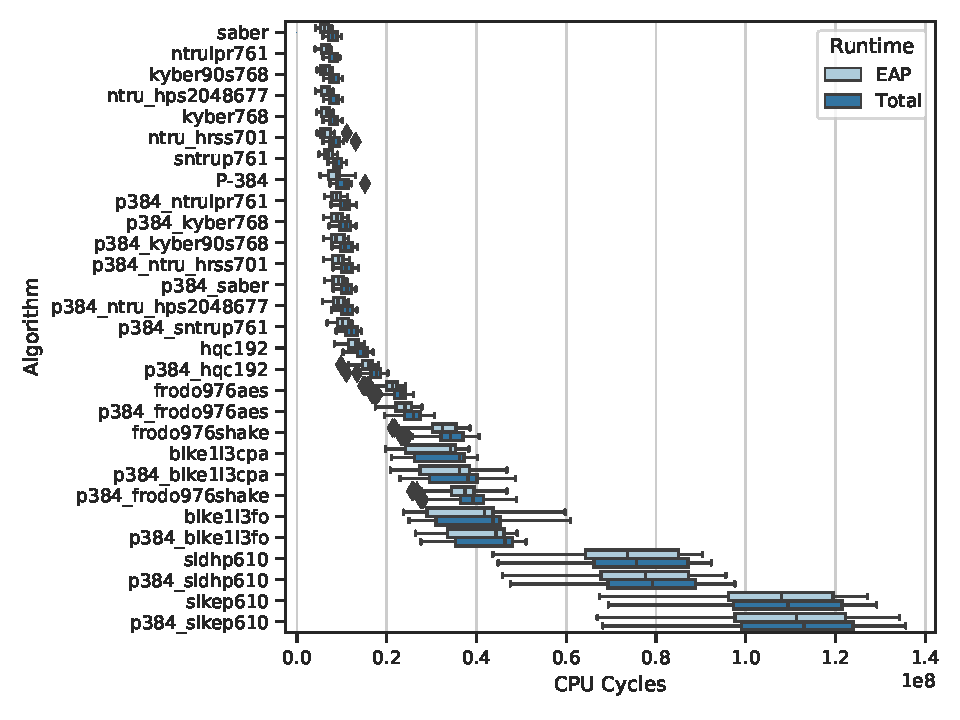
\includegraphics[width=1.0\linewidth]{plot_box_total_runtime.pdf}
    \caption{Total runtime of a single key exchange in \acs{CPU} cycles. The bar represents the quartiles of the distribution, and the whiskers represent the minimum and maximum. Outliers are detected and marked by a diamond symbol.}\label{fig:plot_box_total_runtime}
\end{figure}


Figure~\ref{fig:plot_box_total_runtime} shows the runtime of the experiment grouped by the runtime for the total execution time of the binary and the total execution time of the \ac{EAP} subroutine. The graph shows a clear dependency between both values since the total runtime of the experiment is dominated by the time it takes for a complete \ac{EAP} authentication. The difference between both values is due to the overhead to set up the configuration of the execution and the cleanup routine at the end of the execution. Both values reassemble the values from the ROBOCOP benchmark presented in Chapter~2. Since the figure only shows the \acs{CPU} time spent by the process, the predicted overhead for the request-response design of \ac{EAP} is not visible and the \acs{CPU} time spent is dominated by the runtime of the \ac{KEM} rather than by the amount of traffic. 

\begin{figure}[t]
    \centering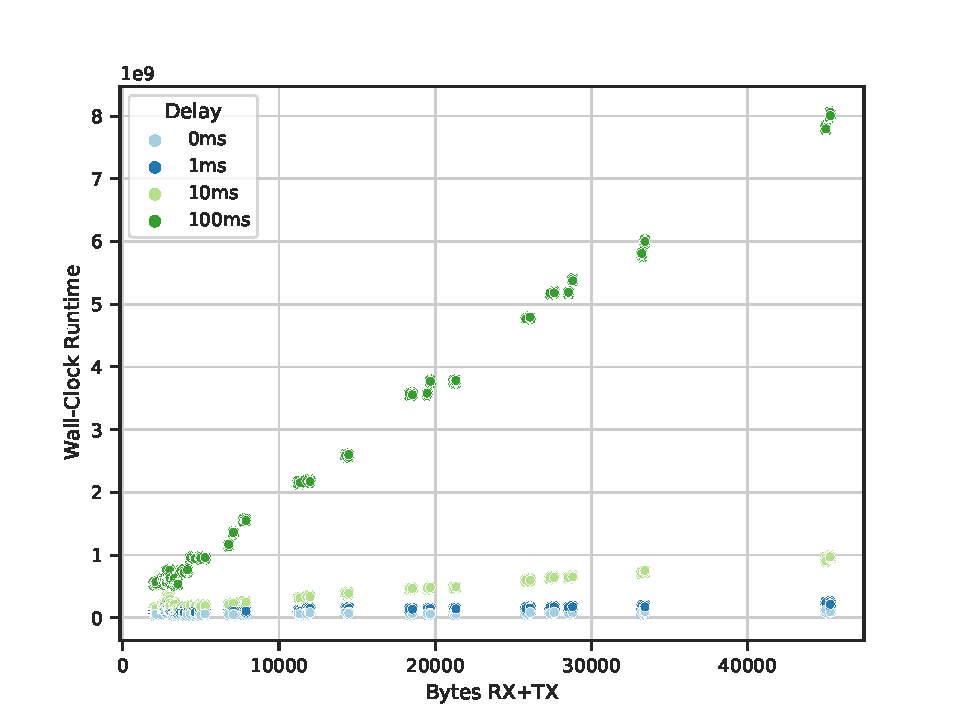
\includegraphics[width=1.0\linewidth]{plot_scatter_handshake_time_vs_traffic_delay.pdf}
    \caption{Total wall-clock runtime of a single key exchange plotted against the total amount of TLS data sent (TX) and received (RX). The delay is an artificial fixed-time delay added to send a message in a single direction.}\label{fig:plot_scatter_handshake_time_vs_traffic_delay.pdf}
\end{figure}

\begin{table}[bh!]
    \caption{Pearson Correlation between the amount of data send and the Wall-Clock Time (WCT), and the \acs{CPU} time spent with different amount of network delay. The last column shows the average wall-clock runtime in seconds.}     
    \begin{center}
        \begin{tabular}{rrrr}
            \hline
            \textbf{Delay} & \textbf{WCT} & \textbf{\acs{CPU} Time} & \textbf{WCT/Seconds} \\
            \hline
            Data & 0.147101 & 0.134977 & 0.132811 \\
            \hline
            \(1ms\) Data & 0.634502 & 0.193965 & 0.162495 \\
            \hline
            \(10ms\) Data & 0.985996 & 0.182698 & 0.341885 \\
            \hline
            \(100ms\) Data & 0.998727 & 0.178201 & 2.026868  \\
            \hline
        \end{tabular}
    \end{center}
    \label{table:peason_delay}
\end{table}


This gets clearer when looking at the wall-clock runtime of a single authentication. Additionally, the experiments run in a local environment with little to no network delay. Figure~\ref{fig:plot_scatter_handshake_time_vs_traffic_delay.pdf} shows the correlation between the wall-clock runtime of the experiments and the amount of data transmitted in both directions. For this experiment, an artificial network delay was added. A delay of \(x\) ms means that \(x\) milliseconds of network delay were added for the transmission in a single direction. This results in \(2*x\) milliseconds total delay for a single round trip. The graph clearly shows a strong correlation between the total runtime of the experiment and the amount of data sent.




Table~\ref{table:peason_delay} makes this dependency even more clear by showing the calculated Pearson correlation between the amount of data transferred, and the wall-clock runtime and the \acs{CPU} cycles spent by the experiments. The first row shows the coefficient when no artificial delay is added. In this case, no correlation is visible. After a short delay of \(1ms\) is added, a clear correlation with the wall-clock time is visible. This gets even more significant with a delay of \(10ms\). In this case, the runtime is already almost completely influenced by the amount of traffic.


\begin{figure}[t]
    \centering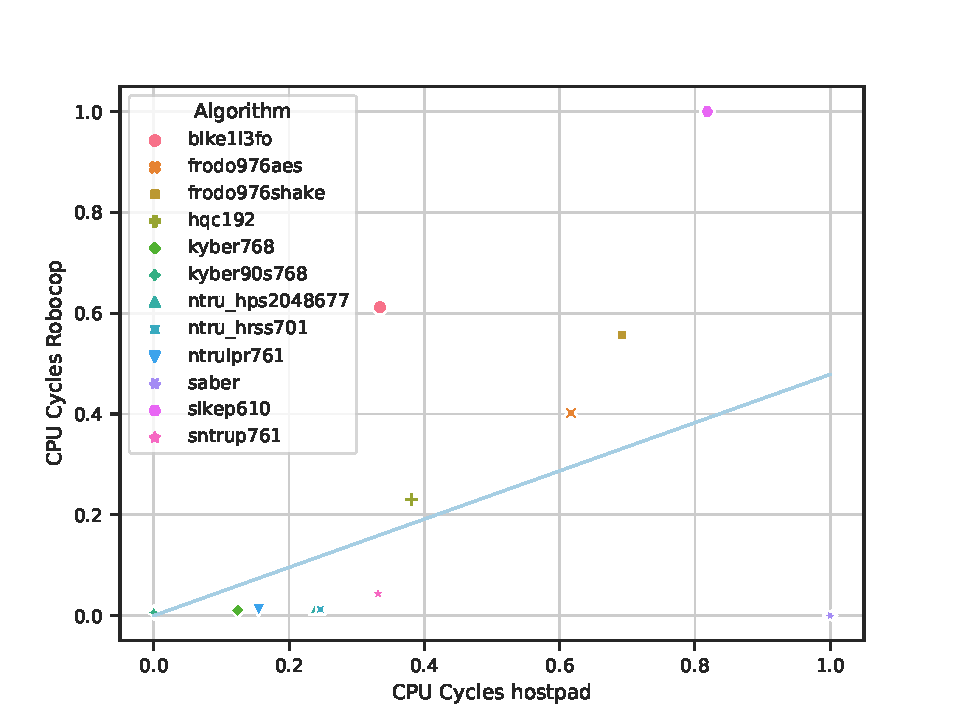
\includegraphics[width=0.8\linewidth]{plot_scatter_robo_eapoltest.pdf}
    \caption{Regression plot of execution times for \ac{PQ} algorithms. The y-axis shows the 50th percentile of the ROBOCOP benchmark runtime in CPU cycles. The x-axis shows the runtime of the experimental evaluation in CPU cycles. The values are calculated using \(log_{10}\) and normalized to \([0,1]\) for visualization purposes.}\label{fig:plot_scatter_robo_eapoltest.pdf}
\end{figure}


When no network delay is present, the runtime of a single \ac{EAP} authentication is dominated by the runtime of the key exchange algorithm. Figure~\ref{fig:plot_scatter_robo_eapoltest.pdf} shows a correlation plot between the mean number of CPU cycles for a single key exchange in the experiments and the number of CPU cycles to generate a single key pair plus a single decapsulation operation according to the robocop benchmark suite. The time to encapsulate a key is not included since this happens on the server-side, which is not included in the execution time on the client. The plot shows that there is a strong linear correlation between the runtime measured by ROBOCOP and the experiments. This gives some confidence in the correctness of the measurements and shows that without network delay, the runtimes of the cryptographic primitives are indeed a dominating factor of the overall runtime of the experiments. The line is a computed regression line between both measurements. While the line shows no perfect correlation (i.~e. \(f(x) = y\), the slope shows a clear linear dependency between both variables.

To get a sense of the runtime, including the computation time spent on the server, Figure~\ref{fig:plot_box_handshake_type_time.pdf} shows the total runtime until a certain point in the TLS handshake is reached. For the visualization of the data, different steps in the handshake were grouped. ``client hello'' reflects the time until the TLS Client Hello message is sent and includes the time for key generation. ``server hello'' reflects the time until the TLS Server Hello message is received by the client and includes the time to encapsulate a shared secret on the server-side. ``finished'' reflects the time until TLS Finished message is received. 


Between the ``Server Hello'' and the ``finished'' message, certificates are exchanged and verified by both the client and the server and include the time to decapsulate the shared secret on the client. An interesting observation is that in some cases, the \ac{PQ} ciphers perform even faster than a classical cipher with the same security level. This is partly due to statistical variances in the measurements and partly due to using data with no delay. This neglects the role of the delay in the total runtime. In cases with an artificial delay of \(10ms\), the classical cipher is the fastest even after considering statistical errors within a small margin.

\begin{figure}[t]
    \centering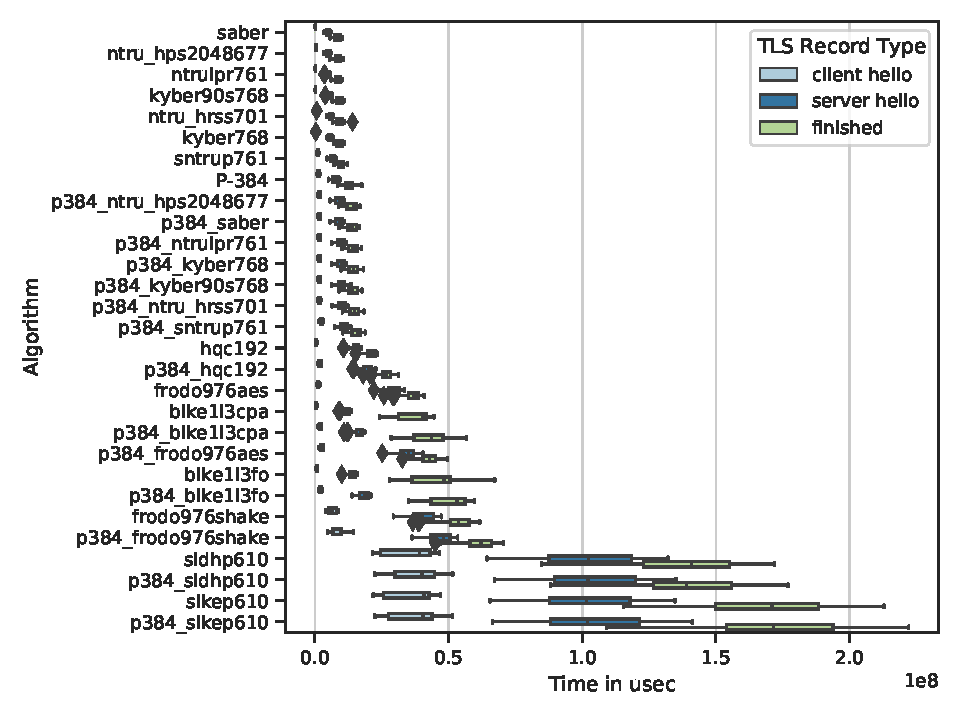
\includegraphics[width=0.8\linewidth]{plot_box_handshake_type_time.pdf}
    \caption{Total wall-clock runtime of a single key exchange, grouped by progress in the TLS handshake. The bar represents the quartiles of the distribution, and the whiskers represent the minimum and maximum. Outliers are detected and marked by a diamond symbol.}\label{fig:plot_box_handshake_type_time.pdf}
\end{figure}

\subsection{Traffic Evaluation}

For the evaluation of the traffic pattern, only \ac{PQ} algorithms will be considered. The reason is that using a hybrid algorithm only adds a rather small overhead of few bytes for the corresponding \ac{ECDH} key exchange to the overall traffic. Figure~\ref{fig:plot_box_traffic_classic_vs_pq.pdf} shows the overall amount of traffic sent for every key exchange with security level 3 in a hybrid and non-hybrid setting. The plot shows that there is only a small cap between both settings, and a numerical evaluation shows an overhead of about 300 bytes for using the \ac{NIST} P-384 curve as an additional classical algorithm. This is about a factor of \(0.04\) additional traffic on average. Since this additional traffic is a small constant overhead, it will be ignored in the remainder of the traffic evaluation for a cleaner visualization.
\begin{figure}[t]
    \centering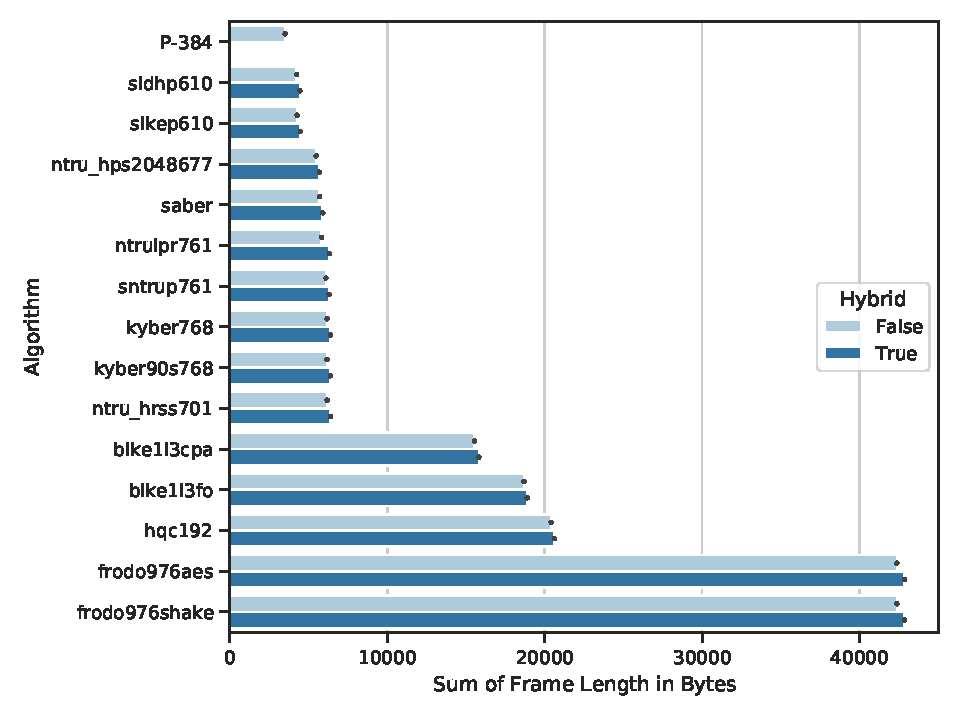
\includegraphics[width=1.0\linewidth]{plot_box_traffic_classic_vs_pq.pdf}
    \caption{Average amount of traffic sent for a single key exchange. The different bars represent whether a hybrid or \ac{PQ}-only variant was used.}\label{fig:plot_box_traffic_classic_vs_pq.pdf}
\end{figure}

Since RADIUS/EAPOL only supports rather small packet sizes, messages are usually fragmented in multiple frames. In the evaluation, fragmentation can occur in multiple protocol-levels. First, the transmitted TLS records need to be sent in different \ac{EAP} Packets. The size of a single \ac{EAP} message is limited to \(1.400\) bytes. Secondly, the \ac{EAP} fragments exceed the size of a single RADIUS \ac{AVP}, resulting in additional fragmentation of the \ac{EAP} Packet in multiple 255-byte long RADIUS \acp{AVP}. Since every fragmentation adds additional overhead to the communication, Figure~\ref{fig:plot_bar_traffic2.pdf} shows the amount of traffic grouped by the different protocols. The first notable observation is that the fraction of EAP-TLS traffic to the total amount of traffic gets smaller as the number of total traffic increases. This is a result of the mentioned fragmentation since every RADIUS packet adds a rather large boilerplate of redundant accounting information. Figure~\ref{fig:plot_avp.pdf} provides an overview of the sources of different overheads in network communication. In this plot, the ratios of different protocol levels are displayed. In the first group, the amount of actual TLS traffic on the overall sent amount of bytes is plotted. In the second category, the ratio of \ac{EAP} traffic in RADIUS AVP values to the overall amount of AVP messages is shown. The last category shows the ratio of TLS traffic to actual \ac{EAP} traffic. The plot shows that the ratio of actual TLS to \ac{EAP} traffic and the ratio of AVP Values to RADIUS traffic is \(> 0.95\). On the other hand, the ratio of TLS to the total amount of traffic is rather low and about \(25\%\) of traffic is due to overheads in the RADIUS layer. Figure~\ref{fig:plot_avp_attr.pdf} shows a detailed overview of the mean amount of AVP traffic for a single key exchange, without the AVP messages used for EAP.

\begin{figure}[t]
    \centering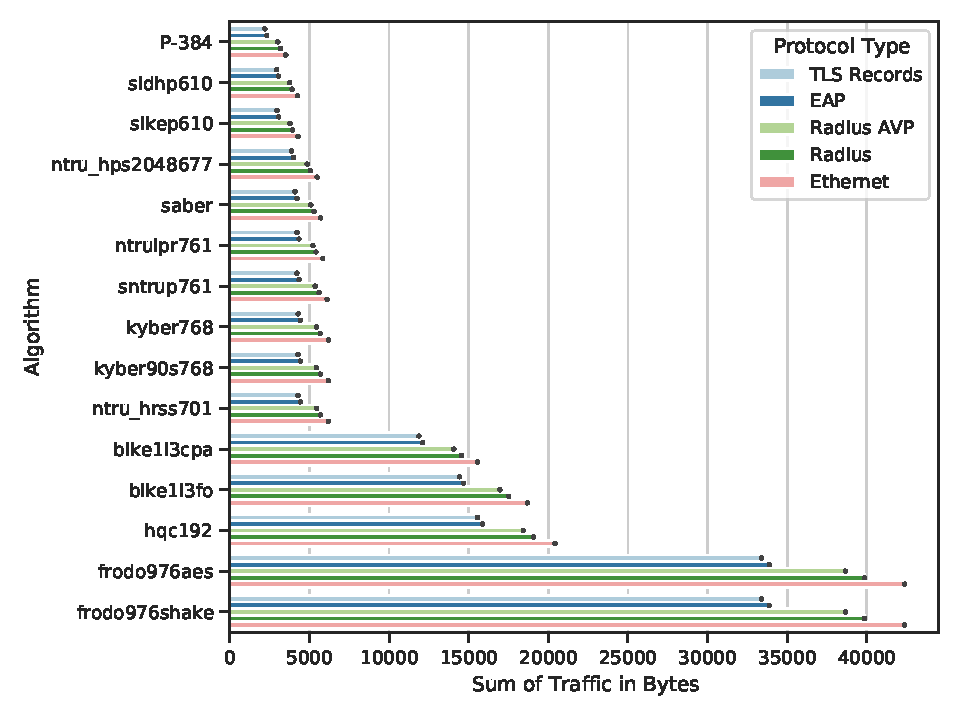
\includegraphics[width=1.0\linewidth]{plot_bar_traffic2.pdf}
    \caption{Amount of traffic for a single key exchange grouped by the type of traffic.}\label{fig:plot_bar_traffic2.pdf}
\end{figure}
\begin{figure}[t]
    \centering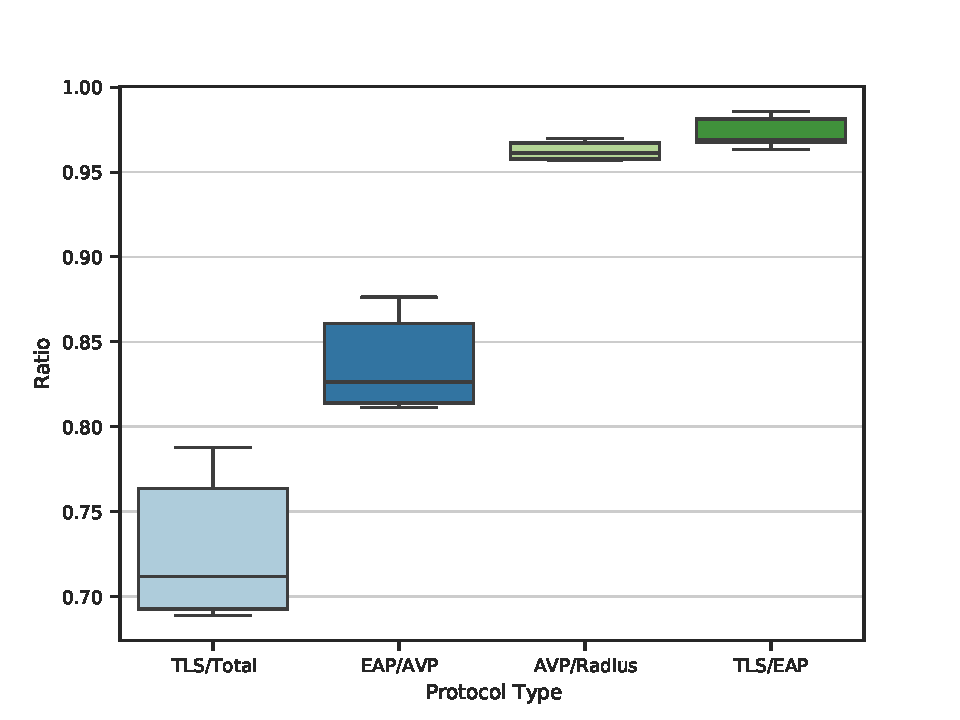
\includegraphics[width=1.0\linewidth]{plot_avp.pdf}
    \caption{Overhead of traffic, expressed as a ratio of different traffic types. \(A/B\) correspondence to the ratio of the traffic of type \(A\) to the traffic of type \(B\). A value close to 1, therefore, indicates little overhead for the encapsulation of the protocols.}\label{fig:plot_avp.pdf}
\end{figure}
\begin{figure}[t]
    \centering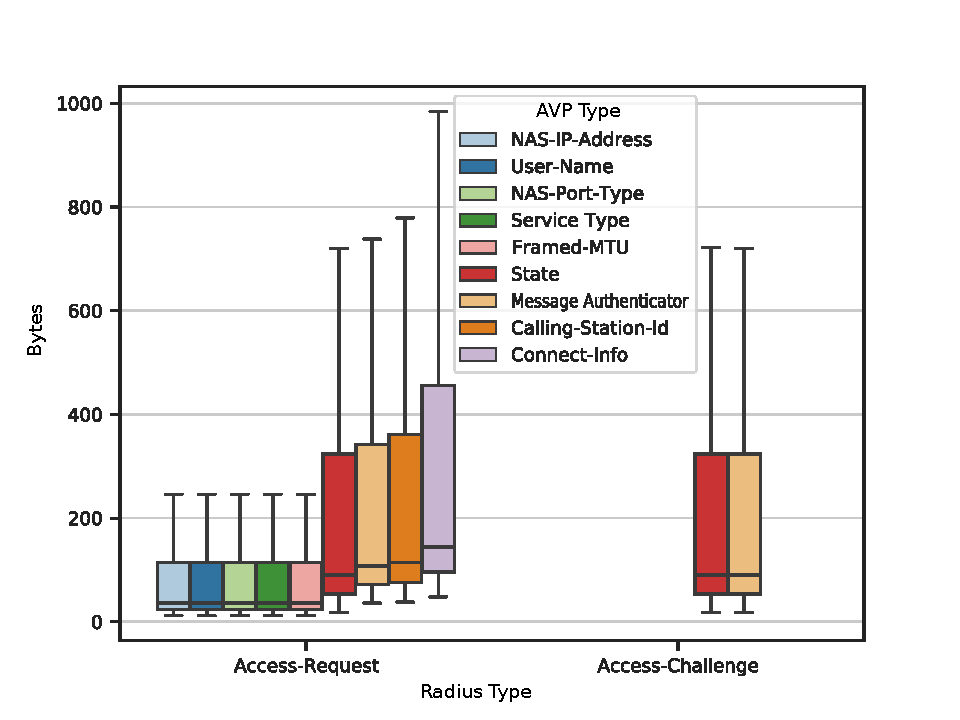
\includegraphics[width=1.0\linewidth]{plot_avp_attr.pdf}
    \caption{Amount of AVP traffic generated by attribute types. The plot is divided into Access-Challenge and Access-Request RADIUS messages. The boxes show the amount of traffic generated for sending the corresponding attribute.}\label{fig:plot_avp_attr.pdf}
\end{figure}

The figure shows that a large amount of traffic occurs for non-\ac{EAP} related attributes. Some attributes are further limited to certain RADIUS types. RADIUS messages of type ``Access-Request'' are sent from the client to the RADIUS server and are acknowledge using a RADIUS ``Access-Challenge'' packet. The ``Access-Accept'' type is used at the end of the \ac{EAP} authentication as a final acknowledgment. The following RADIUS attributes were included in the raw packet captures:

\begin{itemize}
    \item \textbf{NAS-Port-Type} This value is a mandatory value that needs to be included in all ``Access-Request'' messages and identifies the physical port type of the Authenticator. Either this or the ``NAS-Port'' attribute needs to be included.\cite{rfc2865}
    \item \textbf{User-Name} This optional attribute indicates the username of the \ac{EAP} Peer. For RADIUS/EAP, this is the value that is reported by the EAP-Identity packet sent by the Peer.
    \item \textbf{NAS-IP-Address} This attribute identifies a unique IP-address of the Authenticator. Either this or a NAS-Identifier attribute is mandatory by RFC~2869\cite{rfc2869}
    \item \textbf{Framed-MTU} This optional attribute is a hint by the Authenticator to the server and states a preferred MTU size. The server is free to choose whether to honor this request.\cite{rfc2865} 
    \item \textbf{Service-Type} This attribute indicates the type of service the user wants to use. For \ac{EAP}, this is usually fixed to ``Framed'' and is optional.
    \item \textbf{State} This is a response attribute sent by the server to the Authenticator and must be returned unmodified by the Authenticator. The usage of this AVP is not further defined by RFC~2869\cite{rfc2865}. However, it is defined by RFC~5080 to distinguish between a restarted and ongoing session by a Peer.
    \item \textbf{Message-Authenticator} This attribute is mandatory and used for integrity protection of the RADIUS messages. EAP-TLS is integrity protected by itself but is scoped to the TLS handshake and, therefore, an authentication of the RADIUS messages is needed to ensure that the RADIUS messages are not altered.
    \item \textbf{Calling-Station-Id} This AVP identifies the Peer by its hardware address. Since the identity of the Peer is already included in the User-Name attribute, this AVP is redundant.
    \item \textbf{Connect-Info} This AVP includes information on the type of connection the Peer uses to connect to the Authenticator. It includes the type of the link and further information such as the link speed\cite{rfc2869}.
    \item \textbf{Vendor Specific} This attribute contains vendor-specific information. In this case, the value includes Microsoft MPPE-Send-Key and MPPE-Recv-Key messages for compatibility with the Microsoft Point-to-Point encryption protocol and includes a shared secret value\cite{rfc2548}.
\end{itemize}

Overall only the following attributes are mandatory: NAS-Port-Type, User-Name, NAS-IP-Address, Message-Authenticator, State. Figure~\ref{fig:plot_avp_grouped.pdf} shows a comparison of the amount of traffic used for mandatory attributes to the amount of traffic used for optional attributes in the left plot. It shows that up to \(50\%\) of AVP traffic is unnecessary and can be removed. On the right side plot, the figure shows a comparison between the average amount of AVP traffic for two settings. In the ``Full'' setting, all AVP attributes as described above are included. In the ``Sparse'' setting, only the necessary attributes are included. The plot shows that a rather large amount of overhead can be removed. This is beneficial for algorithms with large key sizes, where many RADIUS messages need to be sent.

\begin{figure}[t]
    \begin{subfigure}{\linewidth}
        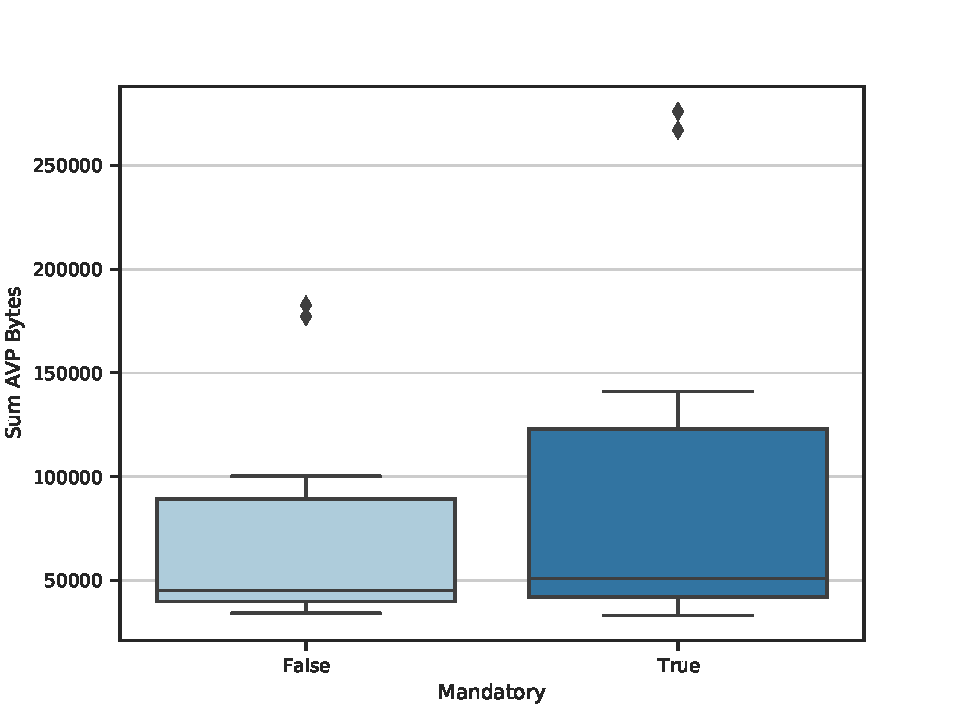
\includegraphics[width=0.49\linewidth]{plot_avp_grouped.pdf}
        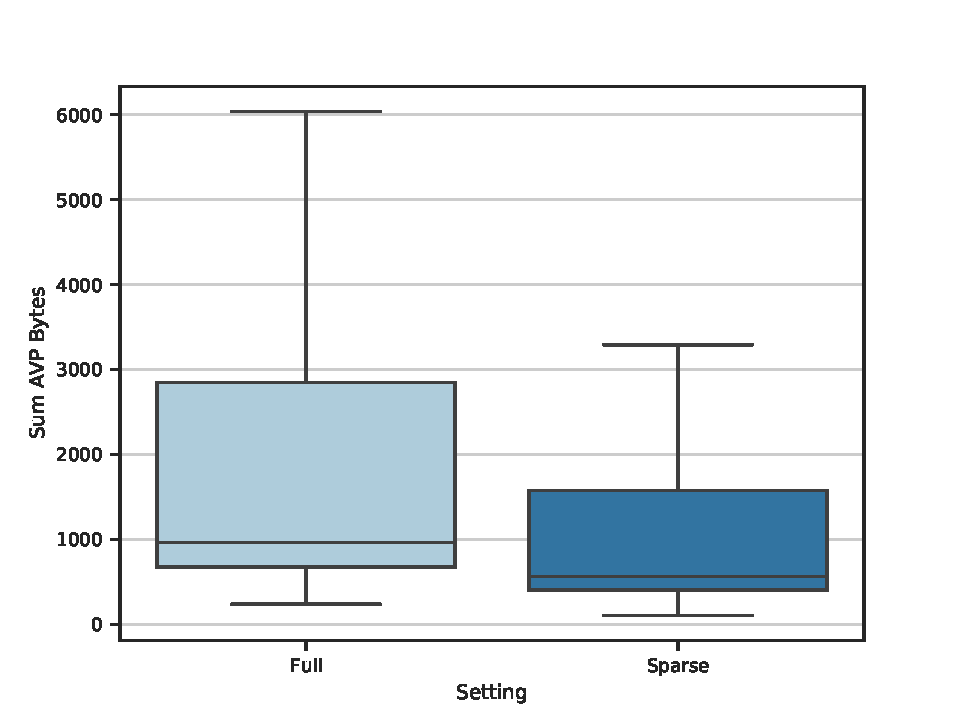
\includegraphics[width=0.49\linewidth]{plot_avp_sparse.pdf}
    \end{subfigure}\caption{Amount of traffic generated by RADIUS AVP attributes in Bytes. The left plot shows the amount of mandatory vs. the amount of optional AVP traffic. Mandatory traffic includes all AVP attributes that need to be sent for EAP-RADIUS to work correctly. Optional attributes include additional billing information that is of no further relevance for a simple key exchange. The right-sided plot shows a boxplot of the amount of traffic in the sparse setting and in the full setting. In the sparse setting, the protocol is stripped of all optional attributes.}\label{fig:plot_avp_grouped.pdf}
\end{figure}

\subsection{Forward Secrecy}
As already discussed in the previous chapter, it is possible to build a non-forward secrecy-based approach by omitting the call to generate a new key pair and use a pre-generated key pair instead. Figure~\ref{fig:plot_box_static.pdf} shows the time for a single execution of a key exchange with two different settings. In the ``static'' setting, a pre-generated key is copied in every execution. In the ``non-static'' setting, a fresh key pair is generated for every execution. The graph shows almost no difference in execution times for most key exchange algorithms. Table~\ref{table:ttest_static_key} further shows a two-sided t-test for the null hypothesis of identical averages. As already seen in Figure~\ref{fig:plot_box_static.pdf}, for most algorithms, it is not possible to reject the null hypothesis, meaning that there is no statistically significant difference in execution times. The reason is that for most algorithms, only a small amount of computation in the experiment is spent on calculating the actual keys and savings on this part of the computation are within the error bounds. The most notable differences exist in isogeny-based approaches and in \texttt{FrodoSHAKE}. For \texttt{SIDHp610}, the results are of no further relevance since the algorithm is not IND-CCA secure, and therefore a static key re-usage would weaken the cryptosystem. For \texttt{Frodo} and \texttt{SIKE}, the mean difference spent on \acs{CPU} cycles is up to \(30\%\). Overall, there is hardly any difference for most algorithms and the savings may not be worth sacrificing forward-secrecy.

\begin{figure}[t]
    \centering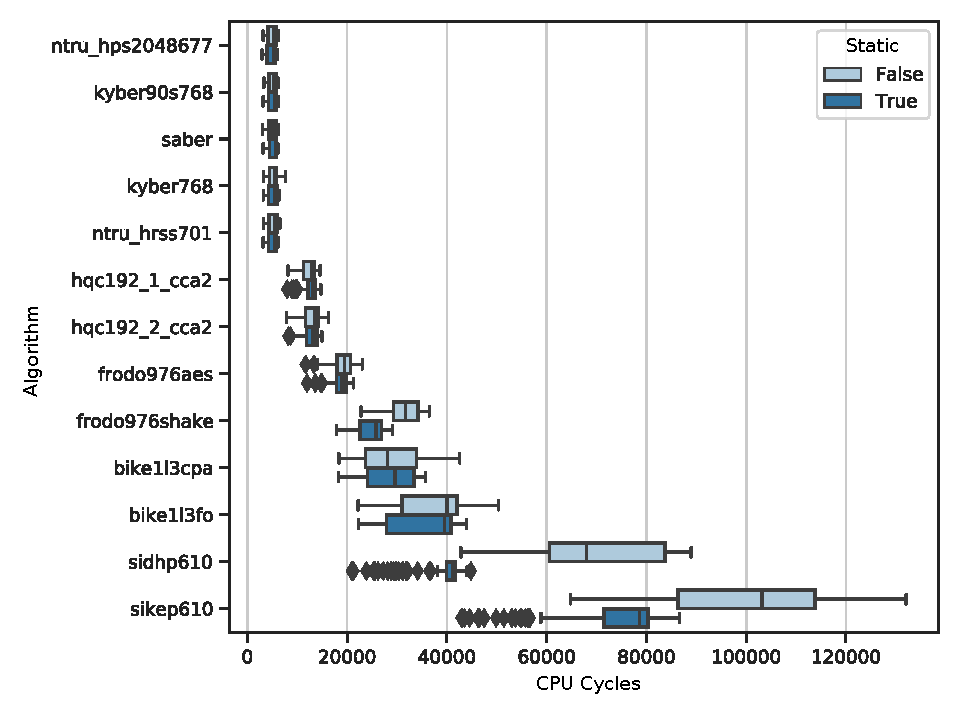
\includegraphics[width=1.0\linewidth]{plot_box_static.pdf}
    \caption{Boxplot of the number of CPU cycles spent for a single key exchange in a static and a non-static setting. In the static setting, a pre-generated key is used for the key exchange. In the non-static setting, a PFS approach is used, where the key pairs are freshly generated for every run.}\label{fig:plot_box_static.pdf}
\end{figure}

\begin{table}[t]
    \begin{center}
        \caption{Difference between the static key and the PFS approach. Mean static is the mean number of CPU cycles for a single key exchange. The mean fresh column is the mean number of CPU cycles for a key exchange with a fresh key for every run. The p-value is the result of a two-sided t-test for identical averages of 100 runs in both settings. A value close to 0 means that the null hypothesis of identical averages needs to be rejected.}     
        \begin{tabular}{lrrrr}
            \hline
        \textbf{Algorithm} & \textbf{Mean static} & \textbf{Mean fresh} & \textbf{p-value}  & \textbf{Difference \%} \\
        \hline
        sidhp610 & \(38424.9\) & \(69788.92\) & \(2.14036282\times 10^{-53}\)&\(-81.62\) \\
        \hline
        frodo976shake & \(24738.31\) & \(31495.17\) & \(5.80376001\times 10^{-36}\) &\(-27.31\) \\
        \hline
        sikep610 & \(73012.13\) & \(99656.51\) & \(9.47968457\times 10^{-27}\)& \(-36.49\) \\
        \hline
        \hline
        ntru-hrss701 & \(5034.1\) & \(5275.87\) & \(0.0588850454705\) &\(-4.8\) \\
        \hline
        hqc192-1-cca2 & \(12693.86\) & \(12328.74\) & \(0.0739710246481\) &\(2.88\) \\
        \hline
        frodo976aes & \(18649.7\) & \(19107.92\) & \(0.0898095252353\)& \(-2.46\) \\
        \hline
        bike1l3fo & \(35057.7\) & \(36726.38\) & \(0.0936540624538\) &\(-4.76\) \\
        \hline
        ntru-hps2048677 & \(4834.48\) & \(5026.03\) & \(0.1477249533302\)& \(-3.96\) \\
        \hline
        kyber90s768 & \(5135.0\) & \(5003.17\) & \(0.2927721808090\)& \(2.57\) \\
        \hline
        saber & \(5165.54\) & \(5052.02\) & \(0.3374748380608\) &\(2.2\) \\
        \hline
        hqc192-2-cca2 & \(12846.73\) & \(12917.97\) & \(0.7592122653455\)& \(-0.55\) \\
        \hline
        bike1l3cpa & \(28813.97\) & \(28643.6\) & \(0.8295043228439\)& \(0.59\) \\
        \hline
        kyber768 & \(5143.36\) & \(5140.64\) & \(0.9834967926456\)& \(0.05\) \\
        \hline
        \end{tabular}
        \label{table:ttest_static_key}
    \end{center}
\end{table}

\newpage
\section{Signature Algorithms}

This section focuses on the evaluation of different signature algorithms. In this setting, the used key exchange algorithm is fixed to the classical \ac{ECDH}-based curve P-384. The evaluation includes all PQ signature algorithms currently available in round 3 of the \ac{NIST} \ac{PQ} project, except for GeMSS, which is currently missing due to license issues\footurl{https://github.com/PQClean/PQClean/pull/326}. The evaluation further focuses on variants with a security level of 3, except \texttt{FALCON}, for which no parameter set with security level 3 is available. In this case, the next higher level 5 is chosen. Hybrid variants additionally use \ac{NIST} curve P-384 with SHA256 as a classical algorithm and P-521 with SHA256 for \texttt{FALCON}. This section will closely follow the evaluation as performed for the key exchange algorithms.

\subsection{Performance Evaluation}

The first evaluation focuses on the overall runtime of the signature algorithms. Figure~\ref{fig:plot_box_total_runtime_sig.pdf} shows the total runtime of a single authentication round, grouped by the total runtime of the experiment and the runtime spent for the actual \ac{EAP} authentication. It is visible that both settings are almost equal in all cases, meaning that most of the time spent on the experiment is actual time spent on the authentication. The graph further shows rather small variances in the error bounds, meaning that the execution time for a single authentication is almost constant. When compared to the runtime of the key exchange algorithms, the amount of time spent on authentication is clearly a dominating factor. The number of CPU cycles spent for a single key exchange ranges from \(4.000\) cycles for \texttt{BIKE} to \(130.000\) cycles for \texttt{SIKEp610}. The authentication time ranges from \(6.000\) cycles for \texttt{dilithium4} to \(3.261.770\) cycles for \texttt{sphincsshake256192ssimple}, with a mean runtime of \(~500.000\) cycles.

\begin{figure}[ht]
    \centering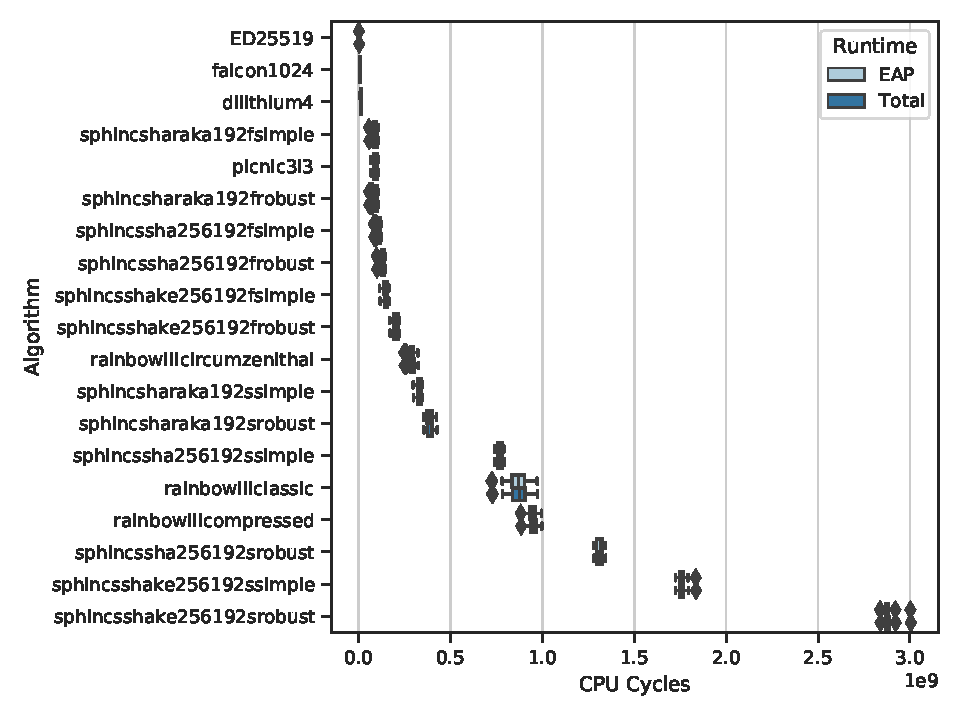
\includegraphics[width=1.0\linewidth]{plot_box_total_runtime_sig.pdf}
    \caption{Boxplot of the number of CPU cycles spent for a single authentication round.}\label{fig:plot_box_total_runtime_sig.pdf}
\end{figure}

Figure~\ref{fig:plot_box_handshake_type_time_sig.pdf} shows a boxplot of the runtime for a single authentication round in wall-clock time, grouped by the states for the TLS handshake. As for the key exchange methods, the runtime in this setting does not depend on the amount of traffic but rather on the actual runtime of the algorithms. \texttt{sphincsshake256192srobust}, for example, uses a significant more amount of \acs{CPU} time compared to \texttt{rainbowIIIcclassic} but needs to transmit 20 times less data for a single key exchange. For the \texttt{client hello} TLS message, the amount of time spent until the message is transmitted is low in almost all cases. One remarkable exception is the \texttt{rainbow} family. Since at this point in the TLS handshake, no signatures are used, this is due to the large sizes of the public keys, which need to be loaded at the start of the experiment. Indeed, a calculation of the Pearson correlation coefficient yields a very strong dependency of over \(0.99\) for the number of \acs{CPU} cycles and the combined size for the public and private keys. Table~\ref{table:cycles_to_keysize_hello} shows the dependency between the key sizes and the increased load times. As the key size increases, the time until the client hello is sent and the server hello is received increases almost linear.

\begin{table}[ht]
    \begin{center}
        \caption{The average number of CPU cycles until either TLS client hello, server hello, or finished message is recorded. Key size refers to the overall size for the public and private key in bytes.}     
        \begin{tabular}{lrrrr}
            \hline
        \textbf{Algorithm} & \textbf{Client Hello} & \textbf{Server Hello} & \textbf{Finished} & \textbf{Key size} \\
        \hline
        dilithium4 & \(6384.71\) & \(8973.87\) & \(10789.73\) & \(15047\) \\
        \hline
        sphincssha256192ssimple & \(6670.89\) & \(16199.79\) & \(759470.87\) & \(23834\) \\
        \hline
        sphincssha256192srobust & \(6501.56\) & \(15981.15\) & \(1299688.44\) & \(23834\) \\
        \hline
        sphincsharaka192ssimple & \(6450.69\) & \(15724.77\) & \(344412.16\) & \(23834\) \\
        \hline
        sphincsshake256192srobust & \(6548.64\) & \(16179.73\) & \(3181622.52\) & \(23834\) \\
        \hline
        sphincsharaka192srobust & \(6451.65\) & \(15878.81\) & \(372063.67\) & \(23834\) \\
        \hline
        sphincsshake256192ssimple & \(6587.52\) & \(16048.19\) & \(1909818.61\) & \(23834\) \\
        \hline
        picnic3l3 & \(6815.40\) & \(21510.97\) & \(70558.27\) & \(37163\) \\
        \hline
        sphincsharaka192fsimple & \(6799.86\) & \(25563.80\) & \(48117.99\) & \(49021\) \\
        \hline
        sphincssha256192frobust & \(6773.12\) & \(25479.43\) & \(106482.23\) & \(49021\) \\
        \hline
        sphincssha256192fsimple & \(6774.90\) & \(25791.80\) & \(81174.88\) & \(49021\) \\
        \hline
        sphincsshake256192frobust & \(6829.87\) & \(25619.42\) & \(195378.33\) & \(49021\) \\
        \hline
        sphincsshake256192fsimple & \(6828.78\) & \(25340.79\) & \(135287.96\) & \(49021\) \\
        \hline
        sphincsharaka192frobust & \(6734.59\) & \(25508.63\) & \(51836.98\) & \(49021\) \\
        \hline
        rainbowIIIccycliccompressed & \(13423.43\) & \(66192.65\) & \(634429.51\) & \(560714\) \\
        \hline
        rainbowIIIccyclic & \(19388.64\) & \(71122.35\) & \(125270.74\) & \(1253211\) \\
        \hline
        rainbowIIIcclassic & \(34170.45\) & \(212697.65\) & \(303599.41\) & \(2617927\) \\
        \hline
        \end{tabular}
        \label{table:cycles_to_keysize_hello}
    \end{center}
\end{table}

\begin{figure}[h!t]
    \centering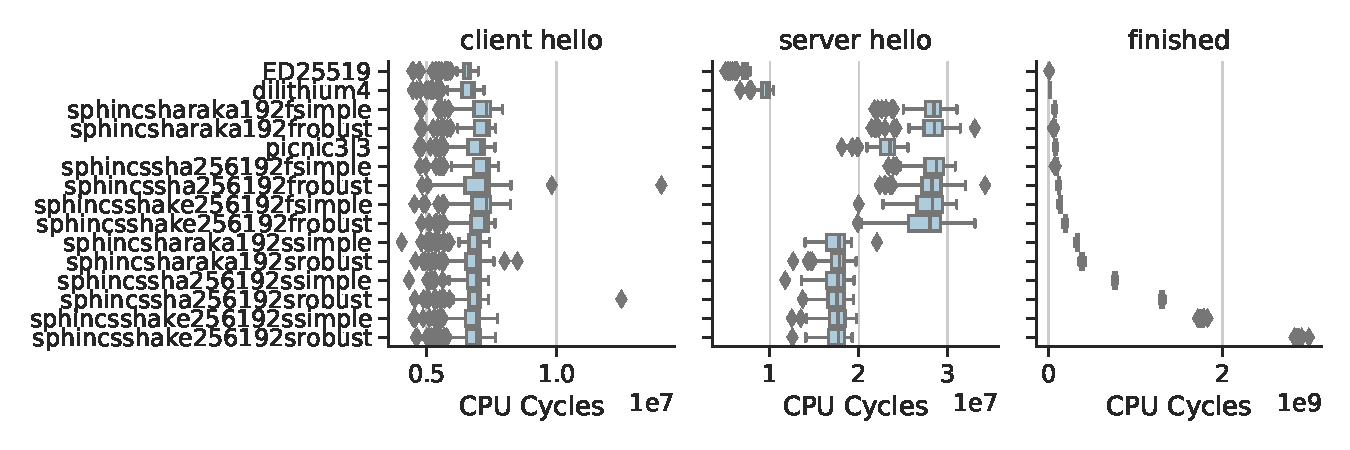
\includegraphics[width=1.0\linewidth]{plot_box_handshake_type_time_sig.pdf}
    \caption{Boxplot of the number of CPU cycles spent for a single authentication round. The different plots show the spent \acs{CPU} time on different stages of the TLS handshake. The ``client hello'' plot displays the point in time when the client hello message is sent, the server hello and finished message represent the time when those messages are received by the client.}\label{fig:plot_box_handshake_type_time_sig.pdf} 
\end{figure}


This changes when taking the time until the TLS finished message is received into account. As visible in Table~\ref{table:cycles_to_keysize_hello}, there seems to almost no dependency between the key size and the time until the TLS finished message is received. As for key exchange algorithms, this only holds in an experimental setting without network delay. If the same experiment as in the last section is performed, where an artificial network delay is added, similar results can be observed. Figure~\ref{fig:plot_scatter_handshake_time_vs_traffic_delay_sig.pdf} shows a scatter plot of different experiments with an increasing network delay added. As already observed for the key exchange methods, the amount of time for a single key exchange increases drastically for algorithms with a large communication pattern as more network delay is added. In contrast to the key exchange algorithms, the effect is not as drastic for the \texttt{SPHINCS} algorithm family. This is because the runtime for this type of signature algorithms is dominated by signature operations even after a delay of 10ms was added. 


\begin{figure}[ht]
    \centering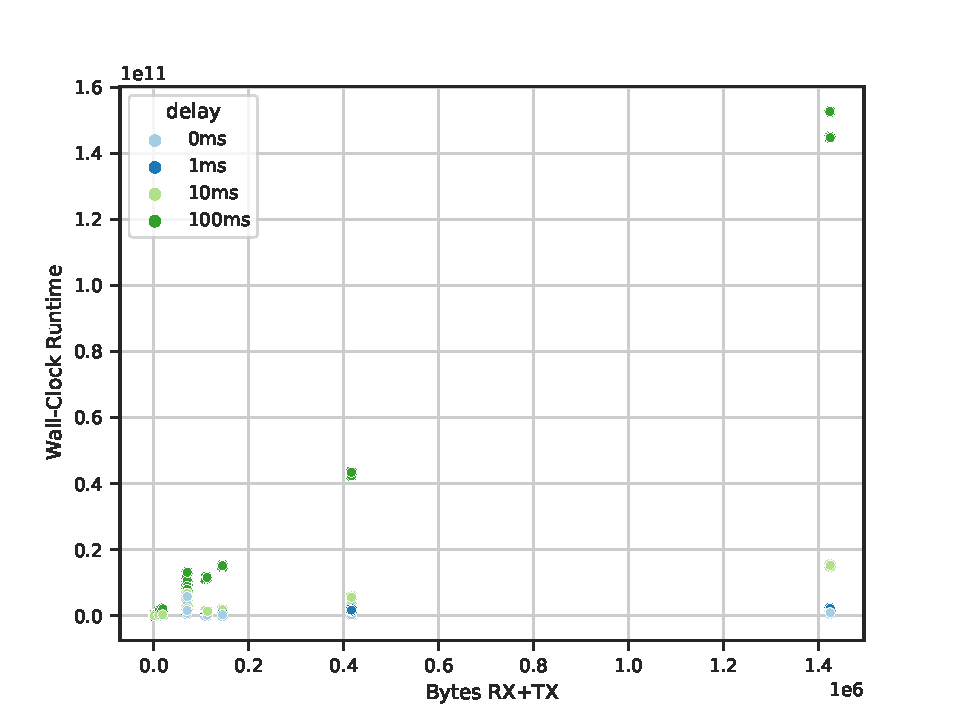
\includegraphics[width=1.0\linewidth]{plot_scatter_handshake_time_vs_traffic_delay_sig.pdf}
    \caption{Scatterplot of the total amount of send and received TLS bytes vs. the amount of wall-clock time spent for a single authentication. The different groups represent different experimental settings with an artificial delay inserted, as described in the last section.}\label{fig:plot_scatter_handshake_time_vs_traffic_delay_sig.pdf}
\end{figure}

\subsection{Traffic Evaluation}

Figure~\ref{fig:plot_bar_traffic_sig.pdf} shows an overview of the overall traffic pattern group by the different signature algorithms. As expected, the traffic pattern depends strongly on the keys that need to be transmitted twice for a single key exchange. As already observed in the key exchange algorithms, the ratio of TLS traffic to the overall traffic is between \(70\) to \(85\) percent. The reasons are the same as for the key exchange algorithms. Because of the request-response nature of \ac{EAP} and the resulting fragmentation, larger overall traffic for EAP-TLS messages results in an increased overhead for the transmission and acknowledgment of single \ac{EAP} frames. Table~\ref{table:overhead_tls_total} shows the total amount of traffic, the total amount of TLS record traffic, and the fraction of TLS record traffic to the total traffic, as an indicator for the overhead for a specific algorithm. As already mentioned in the evaluations for the key exchange algorithms, a large part of the AVP fields consists of redundant and unnecessary information. Since the overhead ratio observed in this evaluation is almost identical to the overhead ratio observed in the key exchange evaluations, a similar amount of savings are expected if these non-mandatory AVP fields are removed.

\begin{figure}[t]
    \centering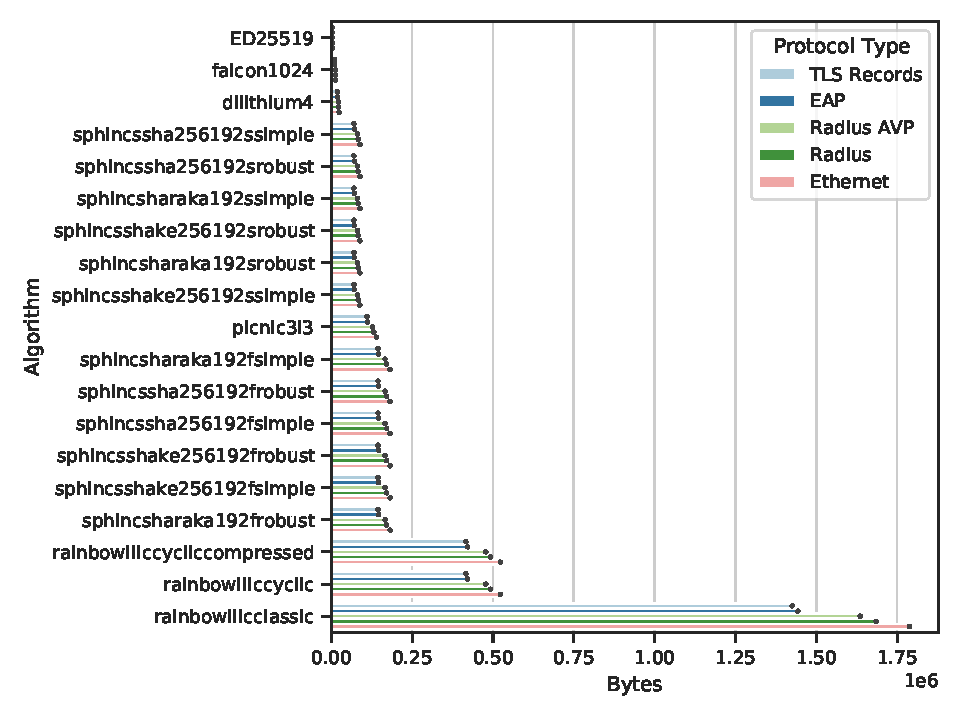
\includegraphics[width=1.0\linewidth]{plot_bar_traffic_sig.pdf}
    \caption{Total amount of sent and received bytes grouped by algorithm and protocol.}\label{fig:plot_bar_traffic_sig.pdf}
\end{figure}


\begin{table}[ht]
    \begin{center}
        \caption{Ratio of send and received bytes for TLS records and overall send and received bytes.}     
        \begin{tabular}{lrrr}
            \hline
        \textbf{Algorithm} & \textbf{Total Bytes} & \textbf{TLS Record Bytes} & \textbf{Overhead}  \\
        \hline
        rainbowIIIcclassic & \(1788120\) & \(1425003\) & \(1.25\) \\
        \hline
        rainbowIIIccyclic & \(522615\) & \(416157\) & \(1.26\) \\
        \hline
        rainbowIIIccycliccompressed & \(522615\) & \(416157\) & \(1.26\) \\
        \hline
        sphincsshake256192fsimple & \(181859\) & \(144511\) & \(1.26\) \\
        \hline
        sphincsshake256192frobust & \(181859\) & \(144511\) & \(1.26\) \\
        \hline
        sphincsharaka192frobust & \(181859\) & \(144511\) & \(1.26\) \\
        \hline
        sphincsharaka192fsimple & \(181859\) & \(144511\) & \(1.26\) \\
        \hline
        sphincssha256192frobust & \(181859\) & \(144511\) & \(1.26\) \\
        \hline
        sphincssha256192fsimple & \(181859\) & \(144511\) & \(1.26\) \\
        \hline
        picnic3l3 & \(139332\) & \(110561\) & \(1.26\) \\
        \hline
        sphincsharaka192srobust & \(88491\) & \(70043\) & \(1.26\) \\
        \hline
        sphincssha256192ssimple & \(88491\) & \(70043\) & \(1.26\) \\
        \hline
        sphincssha256192srobust & \(88491\) & \(70043\) & \(1.26\) \\
        \hline
        sphincsshake256192ssimple & \(88491\) & \(70043\) & \(1.26\) \\
        \hline
        sphincsshake256192srobust & \(88491\) & \(70043\) & \(1.26\) \\
        \hline
        sphincsharaka192ssimple & \(88491\) & \(70043\) & \(1.26\) \\
        \hline
        dilithium4 & \(24089\) & \(18645\) & \(1.29\) \\
        \hline
        falcon1024 & \(13687\) & \(10308\) & \(1.33\) \\
        \hline
        \end{tabular}
        \label{table:overhead_tls_total}
    \end{center}
\end{table}

One interesting observation in Table~\ref{table:overhead_tls_total} is the fact that the overhead ratio seems to increase by a small fraction for protocols with rather small traffic footprints like \texttt{dilithium4} and \texttt{falcon1024}. This seems counter-intuitive but is due to the overhead caused by the initial EAP-Identity and the final EAP-Success message. Usually, this is only a small amount of a few hundred bytes and gets less significant as more data is sent.

\subsubsection{Effect of Frame Length}
Due to the fragmented nature and the corresponding overhead and delay caused by this mechanism, the frame length has an important impact on both the amount of traffic and the total runtime of a single authentication. RFC~2865 defines a maximum size of \(4096\) bytes for a single RADIUS packet\cite{rfc2865}. However, RADIUS uses a two-byte length field and, therefore, would also work with messages up to 65 kB. Figure~\ref{fig:plot_box_fragment_time.pdf} shows the impact of the frame size on the runtime of the experiment. Both plots show the average wall-clock runtime of a single authentication round with increased frame sizes. Two left plot shows the runtime without network delay, and the right plot shows the runtime when an artificial delay of \(10ms\) was added to the network. Figure~\ref{fig:plot_box_fragment_size.pdf} shows the amount of traffic send vs. an increasing MTU size. Both plots show a significant positive impact on the runtime and the amount of data send with an increasing frame size used. The traffic savings between an MTU size of \(1.000\) and \(10.000\) bytes is about 0.25, which matches the expectations from the overhead evaluation. However, both plots show a diminishing improvement as the frame size increases linearly. This may be of further interest when choosing an appropriate frame size. A frame-size of \(4.000\) bytes already provides a significant improvement over the usual default value between \(1.000\) and \(1.500\) bytes without interfering with the \(4.096\) byte limit in RFC~2865.

Alternatively, an alternative \ac{AAA} protocol like Diameter could be used. In contrast to RADIUS, Diameter works connection-oriented through using the TCP instead of UDP. Additionally, there is no limit on the maximum size of a single packet. It is important to keep in mind that TCP would introduce additional overhead for packet acknowledgment. Additionally, the maximum size of a single packet is often limited to Ethernet frame size, which is usually about \(1.500\) bytes. This limitation and the connection-oriented nature of Diameter can neglect the benefits of arbitrary large frame sizes. Due to the complex combinatorial effects, an additional variable would introduce in this evaluation and due to the fact that there are additional security implications that would be needed to be taken into account, an evaluation of Diameter is omitted in this work and left as future work.  

\begin{figure}[t]
    \centering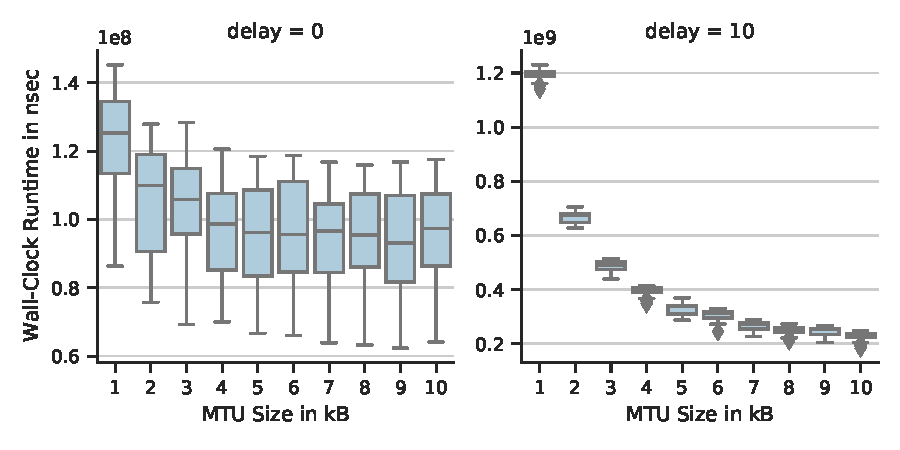
\includegraphics[width=1\linewidth]{plot_box_fragment_time.pdf}
    \caption{Average wall-clock runtime for a single key exchange. The y-axis shows the time in nanoseconds until the TLS handshake is finished and the x-axis shows the used MTU sizes in kB.}\label{fig:plot_box_fragment_time.pdf}
\end{figure}
\begin{figure}[t]
    \centering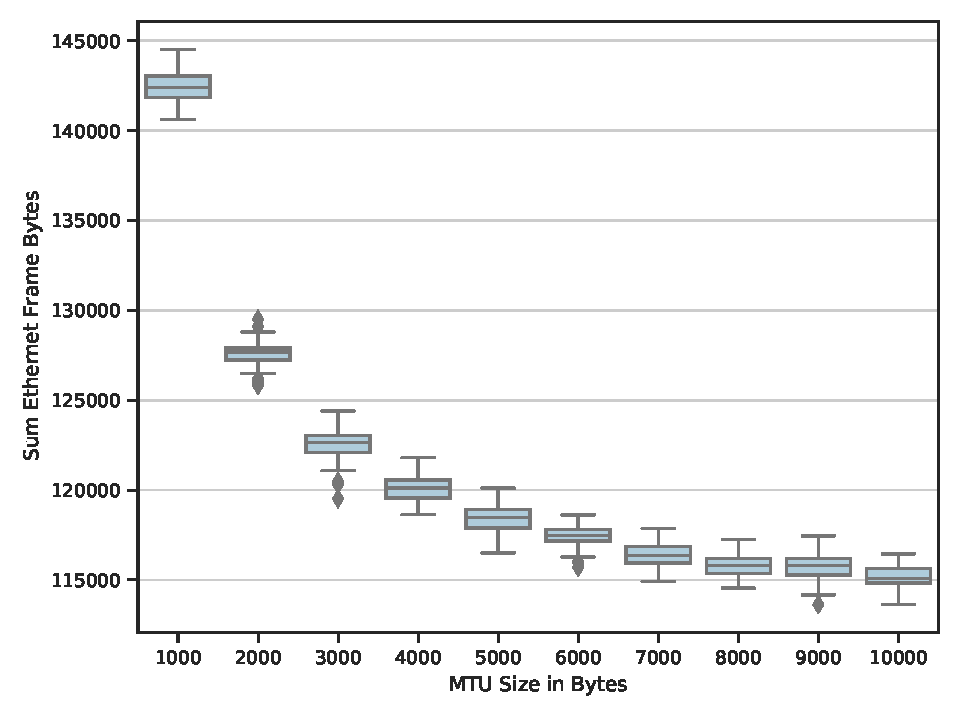
\includegraphics[width=1\linewidth]{plot_box_fragment_size.pdf}
    \caption{Average total amount of data sent to perform a single authentication round. The y-axis shows the sum of the send bytes and the x-axis shows the used MTU/frame size in Bytes.}\label{fig:plot_box_fragment_size.pdf}
\end{figure}

\section{Summary}

In Chapter~4, proposals were made for suitable key exchange and signature algorithms. By combining the results from the raw benchmarks used in Chapter~4 and the experimental evaluation provided in this chapter, it is possible to check the proposals for their practical applicability and further refine the selection of one or more algorithms.

For key exchange algorithms, Kyber and Saber were suitable candidates for both optimized latency and optimized bandwidth. For optimized latency, NTRU and SIKE were selected as additional candidates. When taking a closer look at the evaluation, indeed, it seems that Saber provides the best performance regarding the latency of all evaluated methods. The evaluation further shows that Kyber and NTRU are almost as good as Saber and no statistically significant difference can be shown for these algorithms. For NTRU, this seems surprising when looking at the robocop benchmark, in which a clear difference between NTRU on one side and Kyber and Saber on the other side is visible. This is due to different levels of optimization and different parameter sets of the robocop implementation and the variant used in liboqs. Since all algorithms show similar results, a further look into the traffic evaluation is needed to further refine the selection of the key exchange algorithm. 

When looking at the traffic pattern, it is again possible to confirm the predictions from Chapter~4. Saber, Kyber and NTRU again all have the smallest traffic footprint. As shown in the evaluation, the amount of traffic has a huge impact on the overall runtime of the key exchange due to the fragmented request-response nature of the encapsulation RADIUS/EAP. For this reason, a small traffic footprint is more important than initially stated in the design. The similarity of the results makes it hard to select a clear winner out of the possible protocols. This is also reflected in the announcement of the third round of the \ac{NIST} \ac{PQ} project, which includes all three algorithms as final candidates for the evaluation. Since the results of the measurements are almost indistinguishable, a specific pick of any algorithm would almost certainly be biased and therefore is omitted at this point. A further evaluation of the algorithms by the cryptographic research community eventually will show which algorithm withstands the test of time.

Another promising candidate for optimized communication costs was SIKE. While it stands true that SIKE performs exceptionally well traffic-wise, it only provides a small benefit over other protocols while introducing the highest latency costs of all protocols by a large margin. It may be tempting to select SIKE for the promised DH like structure and for forward-secrecy, but it is important to keep in mind that all protocols were evaluated with ephemeral keys, and a DH like structure alone does not justify the selection of SIKE over other protocols.

Regarding signature algorithms, the most important metric defined in Chapter~4 was the communication cost of the algorithms. It was stated that the Falcon and Dilithium families show the lowest traffic footprint of all algorithms. This could be confirmed by the experimental evaluation. While the difference between falcon1024 and dilithium4 may be relatively small, it is nevertheless significant. Additionally, falcon1024 states a security level of 5, while dilithium4 only provides a security level of 3. This gives more confidence in the security of the parameter selection while still providing a smaller traffic footprint. This gets even more relevant when looking into the performance evaluation. While dilithium provides a better mean performance over all experiments, the difference is negligible. This makes falcon1024 a clear winner for an appropriate signature algorithm.

At this point, it is important to emphasize again that the NIST evaluation is an ongoing process and further research may yield different security levels for the parameters evaluated in this chapter or even may render whole algorithm families broken. While it is almost impossible to quantify the abstract concept of maturity for a cryptographic algorithm, a good way is following the trust of established cryptographers on this topic. Therefore the selection of any algorithm in this section is explicitly performance-driven and the author strongly recommends following the results of the \ac{NIST} \ac{PQ} project when in doubt.

\section{Practical Evaluation}

\begin{table}[h]
    \begin{center}
        \caption{Combination of Signature and KEX algorithms used for the practical evaluation with the sizes for the corresponding public keys. The concatenation symbol (\(\vert\vert\)) means that a hybrid method with both algorithms was used.}
        \begin{tabular}{lrrr}
            \hline
        \textbf{Setting} & \textbf{Signature} & \textbf{KEX} & \textbf{Public Key Bytes}  \\
        \hline
        ECDH & P-521 & P-384 & \(517\) \\
        \hline
        RSA & RSA4096 & P-384 & \(1289\) \\
        \hline
        PQ & falcon1024 & Saber & \(3308\) \\
        \hline
        Hybrid & falcon1024 \(\vert\vert\) P-521 & Saber \(\vert\vert\) P-384 & \(3582\) \\
        \hline
        \end{tabular}
        \label{table:pubkeysizes_practical}
    \end{center}
\end{table}

As mentioned in Chapter~1, this thesis is a cooperation between the LMU University Munich and ADVA Optical Networking as a part of the QuaSiModO project. For this reason, a practical implementation of the evaluation was performed in a real-world scenario, using the ADVA software stack. For this practical implementation, two computers located in Munich and in Tel~Aviv used the implementation of the experimental evaluation to perform a post-quantum key exchange and authentication with a RADIUS server located at a virtual machine at the ``LRZ Computing Cloud'' in Munich. As a result of the authentication, a static key can be transferred from the RADIUS server to the endpoints that can be further used to send authenticated, integrity-protected and confidential MACSec frames between Munich and Tel~Aviv. 

In this section, a short overview of the results of this practical evaluation is shown. For the post-quantum part of the protocol, two settings were used. First, a pure post-quantum implementation, using falcon1024 as a signature scheme and Saber as the key exchange mechanism. In the second post-quantum setting, a hybrid cipher is used, which combines falcon1024 with the NIST P-521 \ac{ECDH} curve and Saber with the NIST P-384 \ac{ECDH} curve. The curves were chosen to match the security level of the respective post-quantum algorithm. For comparison, two classical schemes were evaluated in addition. First, a RSA based scheme with 4096 bit security level as the signature algorithm together with the NIST P-384 \ac{ECDH} curve for the key exchange. Secondly, a purely \ac{ECDH} based variant with the NIST P-521 curve as the signature algorithm and the NIST P-384 \ac{ECDH} curve for key exchange. An overview of the used combinations is shown in Table~\ref{table:pubkeysizes_practical}. The mean latency between the Supplicant and the RADIUS server was \(0.86 ms\). Figure~\ref{fig:plot_scatter_practical.pdf} shows a scatter plot of the spent CPU cycles for a single authentication and the amount of traffic. As expected, the classical settings both perform better in terms of CPU cycles and traffic but within a small distance between the Hybrid and the PQ variant. As expected from the evaluation, the traffic gap between the classical and the PQ variants is rather large. The main contributing factor is the size of the public keys as sown in Table~\ref{table:pubkeysizes_practical}. Since both endpoints need to transfer a public key for mutual authentication together with a corresponding signature, the sum of the sent traffic is \((2*pk + 2*sig + \text{overhead})\). Since falcon1024 signatures are about \(1500\) Bytes long, the minimum amount of traffic is at least \(~9000\) Bytes. This leaves about \(3000\) Bytes for additional overhead and the key exchange when compared to Figure~\ref{fig:plot_scatter_practical.pdf}.

\begin{figure}[t]
    \centering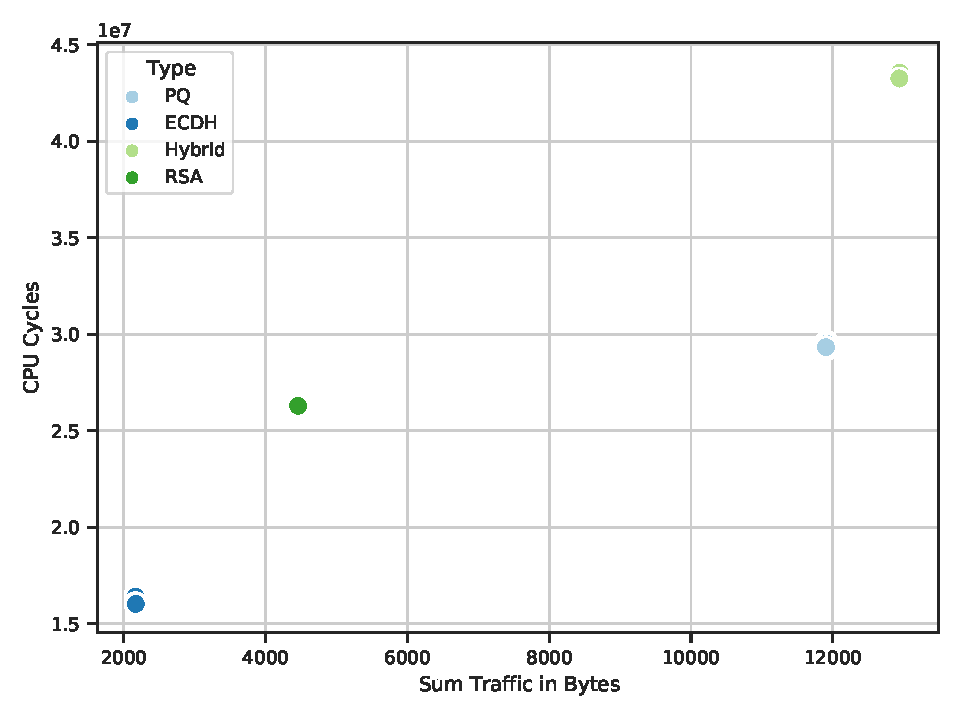
\includegraphics[width=1.0\linewidth]{plot_scatter_practical.pdf}
    \caption{Scatterplot of the total amount of send and received TLS bytes vs. the number of CPU cycles spent for a single authentication. }\label{fig:plot_scatter_practical.pdf}
\end{figure}
When looking at the CPU cycles spent for the mutual authentication, the \acs{CPU} cycles spent for a PQ authentication are about double the time needed for an \ac{ECDH} based authentication. For the hybrid variant, the number of CPU cycles spent closely reassembles the time needed for a PQ authentication plus the time needed for an \ac{ECDH} based authentication. When compared to the RSA based variant, the distance to the \ac{PQ} variant only is within a small margin. While not being as fast as \ac{ECDH} based key exchange and signatures yet, the selected \ac{PQ} variant already reaches values close to classical algorithms. When keeping into account that both Saber and falcon are rather new algorithms, which may not profit from low-level optimization like specifically tailored CPU instructions or highly optimized assembly code, the gap may even become smaller in the future until a point is reached where \ac{PQ} algorithms can replace \ac{ECDH} variants entirely. 

\endinput
